% Тут используется класс, установленный на сервере Papeeria. На случай, если
% текст понадобится редактировать где-то в другом месте, рядом лежит файл matmex-diploma-custom.cls
% который в момент своего создания был идентичен классу, установленному на сервере.
% Для того, чтобы им воспользоваться, замените matmex-diploma на matmex-diploma-custom
% Если вы работаете исключительно в Papeeria то мы настоятельно рекомендуем пользоваться
% классом matmex-diploma, поскольку он будет автоматически обновляться по мере внесения корректив
%
\documentclass{matmex-diploma-custom}
\usepackage{wrapfig}
\usepackage{subcaption}

\begin{document}
% Год, город, название университета и факультета предопределены,
% но можно и поменять.
% Если англоязычная титульная страница не нужна, то ее можно просто удалить.
\filltitle{ru}{
    chair              = {Кафедра системного программирования},
    title              = {Внутреннее представление программ для Transport Triggered Architecture},
    % Здесь указывается тип работы. Возможные значения:
    %   coursework - Курсовая работа
    %   diploma - Диплом специалиста
    %   master - Диплом магистра
    %   bachelor - Диплом бакалавра
    type               = {coursework},
    position           = {студента},
    group              = 242,
    author             = {Ковалёв Дмитрий Александрович},
    supervisorPosition = {},
    supervisor         = {Вербицкая Е.\,А.},
    reviewerPosition   = {},
    reviewer           = {},
    chairHeadPosition  = {},
    chairHead          = {},
%   university         = {Санкт-Петербургский Государственный Университет},
%   faculty            = {Математико-механический факультет},
%   city               = {Санкт-Петербург},
%   year               = {2013}
}

\maketitle
\tableofcontents
% У введения нет номера главы
\section*{Введение}
Параллелизм на уровне команд (ILP) - это способность процессора исполнять параллельно несколько операций. Для реализации ILP процессор должен располагать несколькими \textit{функциональными устройствами (ФУ)}. Общий вид ILP-архитектуры представлен на Рис.~\ref{ilp}.

\begin{figure}[h]
    \centering
    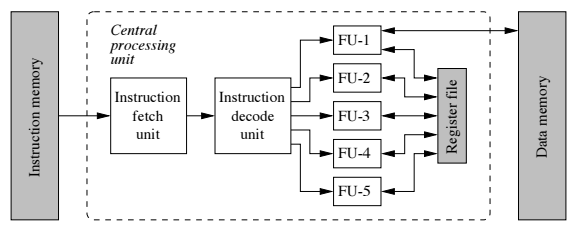
\includegraphics[width=0.7\textwidth]{ilp.png}
    \caption{Общий вид ILP-архитектуры \cite{tta}}
    \label{ilp}
\end{figure}

В настоящее время выделяют три основные ILP-архитектуры: sequential, dependence, independence.

\textit{Sequential} архитектура предназначена для программ, в которых не содержится информация о зависимостях между операциями. Процессор должен выявлять эти зависимости и переопределять порядок операций, чтобы добиться увеличения скорости вычислений. Главным представителем sequential архитектуры являются \textit{суперскалярные} процессоры.

\textit{Dependence} архитектура исполняет программы, в которых, помимо операций, содержится информация о зависимостях между ними. Задачей процессора является нахождение операций, готовых к выполнению, и распределение ресурсов между ними. 

\textit{Independence} архитектура исполняет программы, в которых явно указана информация о том, какие операции могут выполняться независимо друг от друга. То есть, задача нахождения параллельности в программе целиком возлагается на компилятор. Примером такой архитектуры может служит \textit{Very Long Instruction Word (VLIW)} архитектура. Её особенностью является то, что компилятор не только указывает, какие операции могут исполняться независимо, но и распределяет их между ФУ. 

\textit{Transport Triggered Architecture} относится к independence архитектурам. Она схожа с архитектурой VLIW, но, в отличие от неё, требует от компилятора, помимо распределения ФУ, указания каналов, по которым будут перемещаться данные во время выполнения операций. 
% * <Екатерина Вербицкая> 10:32:18 31 May 2015 UTC+0400:
% "Архитектура Transport Triggered Architecture" -- к каждому англоязычному слову нужно русское определяемое.
% ^ <Дмитрий Ковалев> 18:36:49 31 May 2015 UTC+0300:
% Даже если "архитектура ... архитектура"?
\\ \\

Внутреннее устройство TTA (Рис.~\ref{tta}) отличается от стандартной ILP-архитектуры \cite{tta}. ФУ не подключены напрямую к файлу регистров при помощи отдельных каналов. Вместо этого используется сеть с внутрисистемной коммутацией (interconnection network), которая состоит из шин данных и сокетов, устройств для подключения блоков процессора к шинам. Обмен данными между ФУ может проходить напрямую через сеть, без использования файла регистров.

\begin{figure}[h]
    \centering
    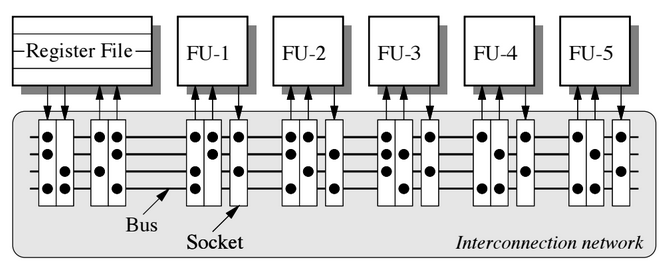
\includegraphics[width=0.7\textwidth]{tta.png}
    \caption{Устройство TTA \cite{tta}}
    \label{tta}
\end{figure}

Основной особенностью TTA является то, что вместо команд, которые должен исполнять процессор, в инструкциях указываются перемещения данных внутри него, а выполнение операций является побочным результатом перемещений. Выполнение операции с $n$ аргументами происходит следующим образом: в регистры операндов соответствующего ФУ помещаются $n - 1$ аргументов, после чего последний аргумент помещается в специальный регистр-триггер, что вызывает начало вычисления.

\textit{Внутреннее представление (ВП)} - это структура данных, удобная для хранения и обработки информации о программе.

\begin{wrapfigure}{r}{0.5\textwidth}
    \vspace{-30pt}
    \begin{center}
        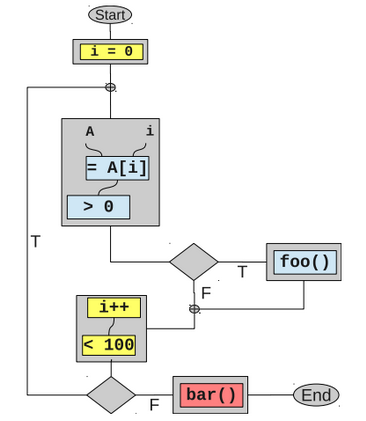
\includegraphics[width=0.4\textwidth]{cfg.png}
    \end{center}
    \vspace{-20pt}
    \caption{Граф потока управления \cite{vsfg}}
    \vspace{-10pt}
    \label{cfg}
\end{wrapfigure}

Наиболее распространенным ВП является \textit{граф потока управления (CFG)} (Рис.~\ref{cfg}). 
Основой такого представления являются базовые блоки - последовательности команд, внутри которых не происходит передачи потока управления. Из базовых блоков и предикатов, контролирующих поток управления, строится искомый граф.

Граф потока управления подходит для использования в компиляторах, которые используются для работы с суперскалярными процессорами, так как последние обладают мощными аппаратными средствами для динамического анализа подобного представления. Примером может служить предсказатель переходов, который с точностью более $95\%$ \cite{vsfg} определяет, к какому базовому блоку перейдет поток управления, и загружает соответствующие команды на конвейер процессора.

К сожалению, данное ВП не подходит для TTA, так как она относится к семейству independence архитектур, то есть, не имеет инструментов динамического анализа. Стандартные средства статического анализа, используемые для подобных архитектур, так же не могут обеспечить высокой эффективности работы TTA, так как особенности устройства графа потока управления мешают им находить независимые операции в программе, снижая уровень ILP \cite{vsfg}.

В данной работе исследовано альтернативное ВП, позволяющее эффективно использовать TTA процессор, приведено описание реализации данного ВП и его интерпретатора.

\section{Постановка задачи}
Целью данной работы является создание и апробация внутреннего представления программ, подходящего для эффективной работы с TTA процессорами. Для её осуществления были поставлены перечисленные ниже задачи.
\begin{itemize}
    \item Изучить альтернативные внутренние представления программ.
    \item Реализовать структуру данных, описывающую необходимое представление.
    \item Реализовать интерпретатор, с помощью которого можно апробировать полученную структуру.
\end{itemize}

\section{Обзор}

В статье Ali Mustafa Zaidi и David Greaves \cite{vsfg} было предложено ВП, обеспечивающее высокую степень параллельности исполнения на архитектурах, не обладающих инструментами для динамического распределения операций. Это ВП получило название \textit{Value State Flow Graph (VSFG)} (Рис.~\ref{vsfg}). Операции в VSFG не разделяются на базовые блоки, и, следовательно, отсутствует понятие передачи потока управления от одного блока к другому. Вместо этого отображаются лишь зависимости между операциями и порядок выполнения операций, имеющих побочные эффекты. Поток управления представлен неявно при помощи вершин-предикатов.  Циклы и вызовы функций являются вложенными подграфами, но со стороны родительского графа выглядят как обычные вершины-операции. 

\begin{figure}[h]
    \centering
    \begin{subfigure}[h]{0.4\textwidth}
        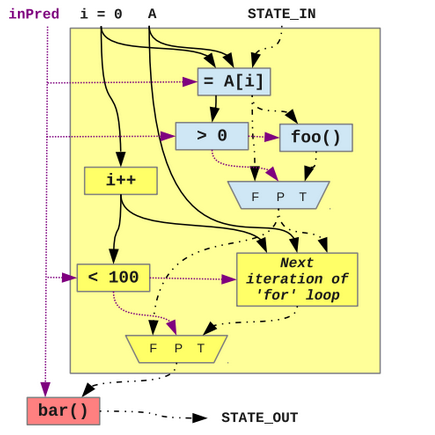
\includegraphics[width=\textwidth]{vsfg.png}
    \end{subfigure}
    \begin{subfigure}[h]{0.5\textwidth}
        \begin{verbatim}
            for (i = 0; i < 100; i++)
                if (A[i] > 0) foo();
            bar();
        \end{verbatim}
    \end{subfigure}
    \caption{Пример кода и VSFG для него \cite{vsfg}}
    \label{vsfg}
\end{figure}
    
VSFG позволяет эффективно распараллеливать итерации цикла, так как подграф, соответствующий итерации, может быть встроен в тело родительского графа. Тем самым, операции из очередной итерации цикла станут доступны для выполнения наравне с остальными. На Рис.~\ref{unrolling} можно видеть пример такой развертки.

\begin{figure}[h]
    \centering
    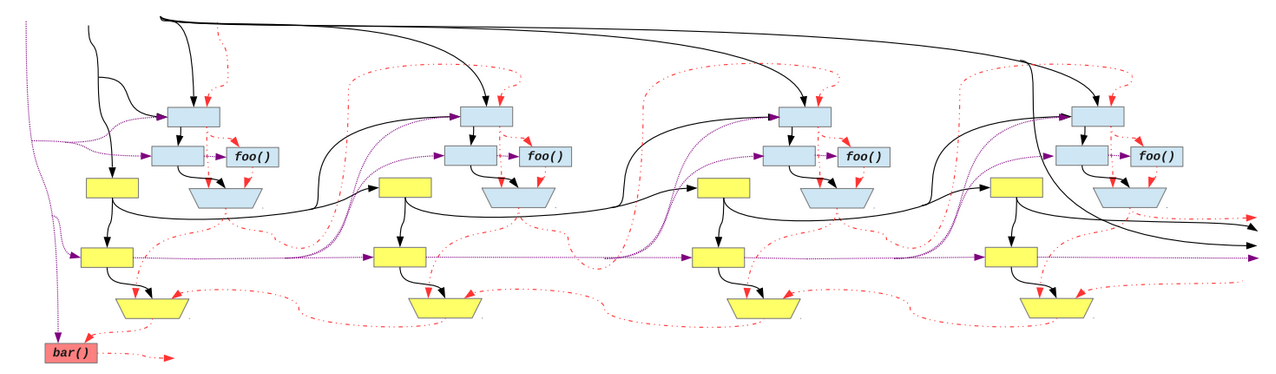
\includegraphics[width=0.9\textwidth]{unrolling.png}
    \caption{VSFG с Рис.~\ref{vsfg}, в котором цикл развернут 4 раза \cite{vsfg}}
    \label{unrolling}
\end{figure}

Еще одним преимуществом данного ВП является возможность одновременного исполнения нескольких регионов кода. В случае использования CFG невозможно, к примеру, перейти к исполнению функции, следующей за циклом, пока цикл не завершится, даже если функция получила все данные, необходимые для её запуска. Такая ситуация возникает из-за использования единственного потока управления. В VSFG такая проблема отсутствует, так как потока управления в явном виде нет, и все операции запускаются сразу после получения данных.

VSFG поддерживают возможность \textit{спекулятивного исполнения}. То есть, операции могут быть запущены до того, как вычислится значение предиката, от которого они зависят. После вычисления предиката ненужные вычисления завершаются. 

\section{Реализация}

\subsection{Структура данных}
Для создания основы структуры, описывающей VSFG, была использована библиотека QuickGraph \cite{quickgraph}. Разработка велась на платформе .NET, язык программирования - F\#. 
VSFG реализован при помощи класса \verb|AdjacencyGraph<Node, Edge<Node>>|. Тип Node представляет собой discriminated union возможных типов вершин графа:
\begin{verbatim}
    type Node =
        | IntVar of IntV
        | Int of int ref
        | Bool of bool ref
        | Pred of Predicate
        | Inc of Increment
        | Div of Division
        | Gate of Multiplexer
        | NextIter of NestedGraph
\end{verbatim}
В данной версии доступно использование переменных типа int (IntV), операций инкремента (Inc) и деления (Div), вершин-предикатов (Pred) и мультиплексоров (Gate). Также возможно реализовать цикл, используя тип NextIter, представляющий собой вложенный граф. 

Тип \verb|Edge<'T>| - стандартный класс библиотеки QuickGraph, используется для связи узлов в графе. Вершины-порты (типы Int и Bool) не связываются дугами с вершинами-операциями, а передаются в конструктор класса операции. Пример такого класса приведен ниже.

\begin{verbatim}
    Division (fst: Node, snd: Node) =
        member this.Ports
        member this.Out
\end{verbatim}

Каждый класс вершин содержит методы Ports (возвращает список портов) и Out (производит вычисления внутри вершины и возвращает результат). 

\subsection{Интерпретатор}
Для апробации структуры был использован пример, приведенный на Рис.~\ref{example}. Для обработки графа интерпретатор использует алгоритм обхода в ширину ~\cite{bfs}. В качестве аргументов основной метод интерпретатора получает граф и набор стартовых вершин. Во время обхода интерпретатор выполняет операцию в вершине, если для неё доступны все входные данные, иначе он помещает ее в конец очереди фронта обхода. Если вершина является вложенным подграфом, то её выполнение запускается в отдельном потоке. Для реализации многопоточности был использован один из стандартных механизмов .NET 4.5~\cite{task}. Вложенные структуры выпоняются спекулятивно, после вычисления значения предиката поток, вычисления в котором нецелесообразны, может быть завершен.

\begin{figure}[t]
    \centering
    \begin{subfigure}[h]{0.3\textwidth}
        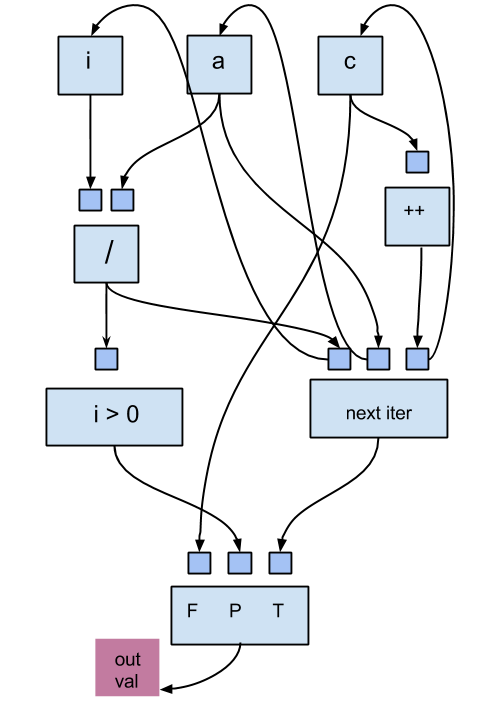
\includegraphics[width=\textwidth]{example.png}
    \end{subfigure}
    \begin{subfigure}[h]{0.6\textwidth}
        \begin{verbatim}
            int func () = 
                int a = 10;
                int c = 0;
                for (int i = 616; i > 0; ){
                    i /= a;
                    c++;
                }
                return c;
        \end{verbatim}
    \end{subfigure}
    \caption{Структура данных для представленного кода}
    \label{example}
\end{figure}

\section*{Заключение}
В рамках данной работы были достигнуты следующие результаты.
\begin{itemize}
    \item Изучено альтернативное внутреннее представление программ (VSFG).
    \item Реализована структура данных, описывающая данное представление.
    \item Реализован интерпретатор, с помощью которого можно апробировать полученную структуру.
\end{itemize}

Исходный код опубликован в репозитории https://github.com/lares77/Brahma.FSharp

Учетная запись автора - lares77.

\bibliographystyle{ugost2008ls}
\bibliography{diploma.bib}
\end{document}
